\documentclass[11pt,english]{article}

\usepackage{pslatex,palatino,avant,graphicx,color,amsmath}

\usepackage [english]{babel}
\usepackage[margin=1.7cm]{geometry}

\begin{document}
\title{ A textual statistical analysis of SEFI 2014 documents}
\author{ Pantelis Z. Hadjipantelis - EDG, UK \\ Sponsor: Joachim Schlosser - Education Marketing, DE}
\date{September 2014}
\maketitle
\vspace{-.61cm}

We aim to provide a coherent statistical analysis of the SEFI (European Society for Engineering Education) 2014 paper submissions. The sample available consists of 133 papers; these papers are provided in .pdf, .doc(x) and .txt formats. We were also provided with an XML document having the papers' title, author(s) and abstract. Analysis is conducted in MATLAB utilizing readily available functionality. The final deliverables are: \begin{itemize}\item Correlation matrix between the most prominent document terms
\item 3-D scatter and surface plot visualizing the main conceptual axes of the conference papers
\item Basic hierarchical clustering of the document terms used
\end{itemize}

We currently utilize the information provided by the XML document only; as such we analyse \textit{only} the papers' abstracts. The basic theoretical background behind the current analysis can be found in : \cite{manning2008introduction,landauer1998introduction}. \\
\textbf{Preprocessing and dataset generation:}
Given the sample of documents we construct a bag-of-words to represent our data.  
Each word is considered an \textit{attribute} and each document a \textit{record} \cite{LaroccaNeto2000a}. 
Basic preprocessing included : 1. Case-folding correction (eg. Student $\rightarrow$ student), 2. Stop-word removal (eg. \textit{do}, \textit{can}, etc.) and 3. Singular/plural reconstruction (eg. students $\rightarrow$ student); this 3rd step can be seen as an extremely basic \textit{stemming} procedure \cite{LaroccaNeto2000a}. 
In a way similar to \cite{xu2003document} we construct a weighted term-frequency vector to represent each document. Assuming that $W = \{w_1, w_2, \dots, w_m\}$ to be the complete vocabulary of our corpus we use an TF-IDF (Term Frequency - Inverse Document Frequency) technique to reweigh our data in terms of how important a word is to a document in the current corpus at hand. We also normalize each vector to have unit magnitude. We did not utilize the complete vocabulary of our corpus; aiming to reduce the dimensions of our dataset and based on the approach used in \cite{fung2003hierarchical} we utilized the first 30 most frequent words (after preprocessing) in our corpus to generate our final matrix $X$. 
\begin{align*}
X_i =& [x_{1i}, x_{2i}, \dots, x_{mi}]^T\\
x_{ji} =& t_{ji} \log(\frac{n}{idf_j})\\
X_i =& X_i / ||X_i||
\end{align*} 
where $t_{ji}$ is the term frequency of the word $w_j$ in document $d_i$, $n$ is the total number of documents analyzed and $idf_i$ the number of documents containing the word $w_j$. Counting, string comparisons and norm normalization can be easily implemented in MATLAB using functions such as \texttt{numel}, \texttt{strcmp} and \texttt{norm}.\\
\textbf{Dataset factorizations and document clustering:}
The two approaches we explore are Latent Semantic Analysis \cite{landauer1998introduction} (a Singular Value Decomposition (SVD) method) and document clustering based on Non-negative Matrix Factorization (NNMF) \cite{xu2003document}. Both methods essentially project a document into a subspace defined by the basis provided by the matrix factorization technique they employ. One then uses standard clustering algorithms on the projected data to find meaningful clusters. The basic difference between the two algorithms is that SVD is not guaranteed to provide positive modes of variation while NNMF does. In that way one avoids the conceptually incoherent concept of negative document values. On the other hand the basis presented by NNMF are not guaranteed to be orthogonal, making the overall dimension reduction less efficient in terms of RSS. In short given a matrix $A_{m \times n}$ in the case of SVD one can produce a factorization:
\begin{align*}
A = U \Sigma V^T
\end{align*}
such that $U$ is an $m \times m$ unitary matrix, $\Sigma$ is an $m \times n$ diagonal matrix of non-negative values and $V$ an $n \times n$ unitary matrix. In the case of NNMF one can produce a factorization:
\begin{align*}
A = WH
\end{align*}
such that both $W$ and $H$ are non-negative matrices of dimensions $m \times k$ and $k \times n$ respectively  minimizing the functional:
\begin{align*}
f(W,H) = \frac{1}{2} || A - WH ||_f^2
\end{align*} 
Computation of both the SVD as well as NNMF procedure are directly available in MATLAB using the functions such as: \texttt{svd} and \texttt{nnmf} respectively. Clustering the documents explores two approaches, a flat clustering approach and a hierarchical clustering approach. The flat clustering approach does not assume any explicit structure relating the cluster; for this we are going to use a \textit{k}-means algorithm. The hierarchical clustering approach implements a hierarchical agglomerative clustering (HAC) methodology that starting from single element clusters merges them together until all elements are part of a single cluster \cite{manning2008introduction}. In both clustering approaches we used a cosine distance metric as it is the most-widely used as well as the most theoretically coherent to the transformation we have conducted \cite{landauer1998introduction,steinbach2000comparison,shahnaz2006document}. Regarding HAC we used a UPGMA algorithm to compute distances \cite{steinbach2000comparison,fung2003hierarchical}.  Computation of \textit{k}-means clustering as well as HAC using a cosine distance is immediately available in MATLAB using the functions \texttt{kmeans} and \texttt{linkage} respectively.\\ 
\begin{figure}[t]
    \centering
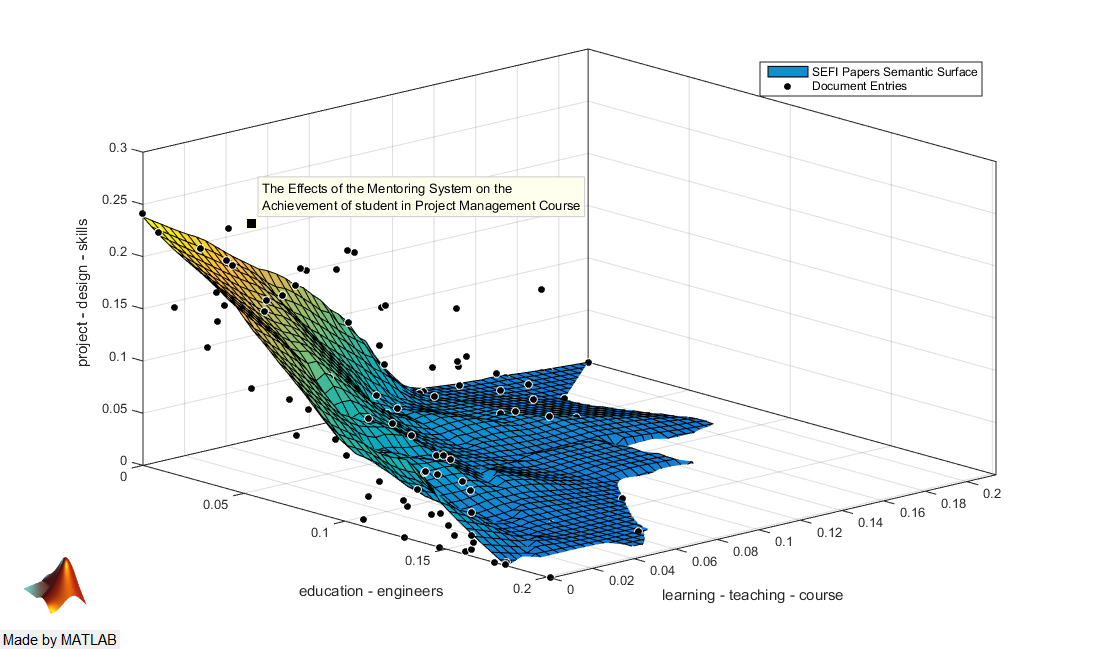
\includegraphics[width=0.98\textwidth]{FinalFigure1858.png}
\caption{The semantic surface defined by the NNMF projected documents.} \label{FIG1}
\end{figure} 
\textbf{Final deliverables:}
Aside the correlation and hierarchical clustering matrices between the keywords we provide an interactive figure where clicking at the data-points returns the document title they are associated with (eg. Fig. \ref{FIG1}). All references are available in the author's public folder.

\bibliographystyle{vancouver}
\bibliography{SEFI_bib}

\end{document}